\documentclass[a4paper,10pt]{article}
%**************************************************************************************************
% PACKAGES
%**************************************************************************************************
\usepackage{amsmath, amsthm, amsfonts, amssymb}
\usepackage{graphicx,color}
\usepackage{bm}	
\usepackage{float}
\usepackage{amstext}
\usepackage{IEEEtrantools}

\LARGE 

%**************************************************************************************************
% DEFAULT SETTINGS
%**************************************************************************************************
\marginparwidth -20 true pt    % Width of marginal notes.
\oddsidemargin  -10 true pt       % Note that \oddsidemargin=\evensidemargin
\evensidemargin -10 true pt
\topmargin -0.5 true in        % Nominal distance from top of page to top of
\textheight 10 true in         % Height of text (including footnotes and figures)
\textwidth 7 true in        % Width of text line.
\parindent=0pt                  % Do not indent paragraphs
\parskip= 1 ex
\columnseprule = 0.1pt
\footskip = 30 true pt
\hoffset = -0.1 true in
\voffset = -0.1 true in
\abovedisplayskip 1 true pt
\abovedisplayshortskip 1 true pt
\topsep 0 true pt

%**************************************************************************************************
% DOCUMENT DETAILS
%**************************************************************************************************

\title{\bf NIS Project Writeup}

\author{Josh Buchalter, Andreas Von Holy, Alon Bresler, Osher Shuman \\
BCHJOS003, VHLAND002, BRSALO001, SHMOSH001 \\\\
Department of Computer Science, University of Cape Town, Rondebosch 7701, \\Cape Town, South Africa.}

%**************************************************************************************************
% MAIN DOCUMENT 
%**************************************************************************************************

\begin{document}
\maketitle

\begin{abstract}
A writeup detailing the implementation details of our secure client-server system.
\end{abstract}

%*********************************************************************************************************
\section{Introduction}
We were tasked with creating a secure client-server communication system that implemented the practices laid out in PGP security. These practices are namely, message confidentiality and authentication. In this writeup, we document the implementation of these practices as well as detailing the choice of language the system is written in, the algorithms used, key management and finally communication connectivity model.
%*********************************************************************************************************
\section{Implementation}
The process of providing message confidentiality and authentication, as laid out in PGP, is shown below and formed the basis for our implementation.

\begin{figure}[H]
\centering
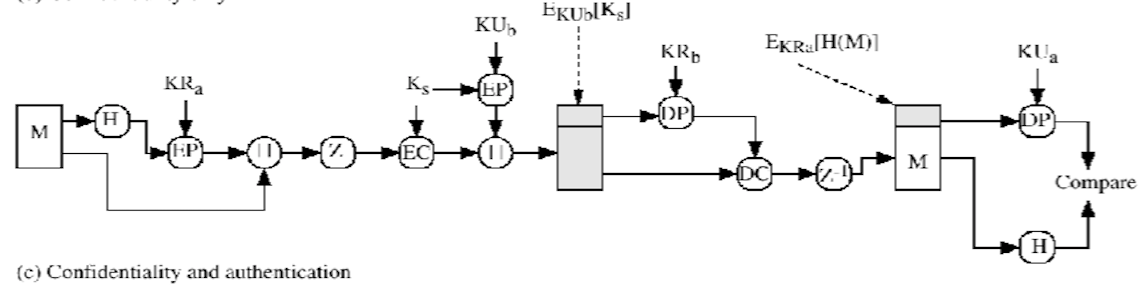
\includegraphics[width=0.7\linewidth]{PGP_Auth_Conf}
\caption{The full PGP process}
\label{fig:PGP_Auth_Conf}
\end{figure}

\subsection{Client}
\begin{figure}[H]
\centering
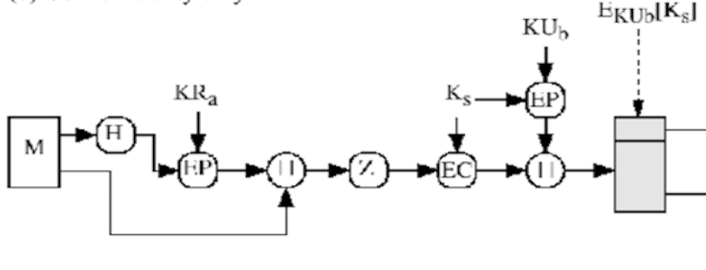
\includegraphics[width=0.7\linewidth]{Client_Side}
\caption{Encryption process done by the client}
\label{fig:Client_Side}
\end{figure}


\subsection{Server}
\begin{figure}[H]
\centering
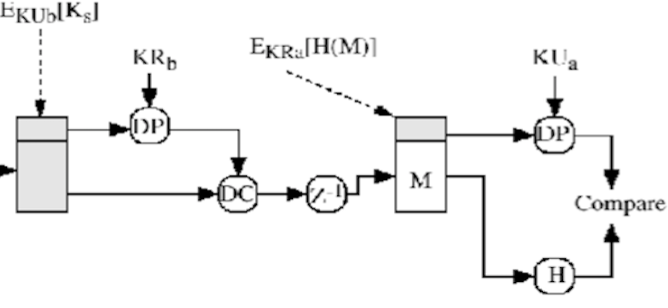
\includegraphics[width=0.7\linewidth]{Server_Side}
\caption{Decryption process done by the server}
\label{fig:Server_Side}
\end{figure}

%*********************************************************************************************************
\section{Choice of Language}
Choice of Language here..
%*********************************************************************************************************
\section{Choice of Cryptographic Algorithms}
The following cryptographic algorithms were implemented.

\subsection{Key Generation}
\subsubsection{Public/Private Key Pair}

\subsection{Encryption}


\subsection{Decryption}
Decryption here...
%*********************************************************************************************************
\section{Key Management}
Key Management here...
%*********************************************************************************************************
\section{Communication Connectivity Model}
Comms connectivity model here...
%*********************************************************************************************************
\section{Conclusion}
Conclusion here.. (if necessary)
%*********************************************************************************************************

%*********************************************************************************************************
% REFERENCES
%*********************************************************************************************************

\end{document}
